% =====================================================================
% Chương 11: Bảo mật đám mây (Cloud Security)
% Bản dịch tiếng Việt đầy đủ từ:
%   Sunilkumar Manvi, Gopal K. Shyam,
%   "Cloud Computing: Concepts and Technologies", CRC Press, 2021,
%   Chapter 11 "Cloud Security", trang 205-227.
% =====================================================================

\chapter{Bảo mật đám mây}

\begin{learningobjectives}
Sau khi đọc chương này, bạn sẽ có khả năng:
\begin{itemize}
  \item Đánh giá bảo mật dữ liệu trong Đám mây (Cloud)
  \item Mô tả quản lý bảo mật trong Đám mây
  \item So sánh và đối chiếu bảo mật IaaS, PaaS, SaaS trong các triển khai Đám mây.
\end{itemize}
\end{learningobjectives}

Bảo mật điện toán đám mây (Cloud computing security) hay nói cách khác là bảo mật Đám mây (Cloud security) ám chỉ một tập hợp rộng lớn các phương pháp tiếp cận, công nghệ và biện pháp kiểm soát được triển khai nhằm bảo đảm thông tin, các ứng dụng và hạ tầng liên quan của điện toán đám mây. Nó là một lĩnh vực con của bảo mật máy tính (computer security), bảo mật mạng (network security) và rộng hơn nữa là bảo mật dữ liệu (data security). Khả năng lưu trữ của điện toán đám mây cung cấp cho khách hàng năng lực lưu trữ và xử lý thông tin của họ trong các trung tâm dữ liệu (data center). Các tổ chức sử dụng Đám mây trong một phạm vi rộng các mô hình dịch vụ (ví dụ, SaaS, PaaS và IaaS) và các mô hình triển khai (riêng tư, lai, công cộng và cộng đồng).

Những mối quan ngại về bảo mật liên quan đến điện toán đám mây rơi vào hai loại: các vấn đề bảo mật mà các nhà cung cấp Đám mây phải đối mặt (những tổ chức cung cấp phần mềm, nền tảng, hoặc hạ tầng dưới dạng dịch vụ thông qua Đám mây) và các vấn đề bảo mật mà khách hàng của họ phải đối mặt (những tổ chức hay hiệp hội có ứng dụng hoặc thông tin được lưu trữ trên Đám mây). Các trách nhiệm được chia sẻ giữa họ. Các nhà cung cấp phải bảo đảm rằng các dịch vụ của họ là an toàn và rằng thông tin cũng như ứng dụng của khách hàng được bảo vệ, trong khi khách hàng phải thực hiện các biện pháp để hỗ trợ các biện pháp bảo mật (chẳng hạn như sử dụng mật khẩu mạnh).

\section*{Các khái niệm sơ bộ}
\addcontentsline{toc}{section}{Các khái niệm sơ bộ}

Sau đây là một số thuật ngữ và định nghĩa được đưa ra ở đây để dễ hiểu hơn trong phần còn lại của chương này.

\textbf{Tính bí mật (Confidentiality)} là sự ngăn chặn việc tiết lộ nội dung một cách trái phép, dù có chủ ý hay không có chủ ý. Việc mất tính bí mật có thể xảy ra theo nhiều cách. Ví dụ, mất tính bí mật có thể xảy ra thông qua việc cố ý phát tán thông tin riêng tư của công ty hoặc thông qua việc áp dụng sai các quyền mạng. Hãy xét tính bí mật của dữ liệu được lưu trữ bởi một hệ thống lưu trữ phân tán. Nếu các tài nguyên đã lưu trữ được phục vụ cho bất kỳ thực thể nào gửi yêu cầu, thì tính bí mật của dữ liệu vốn được dự định chỉ có thể truy cập bởi một tập con người dùng cụ thể sẽ không thể được bảo đảm.

\textbf{Tính toàn vẹn (Integrity)} là sự bảo đảm rằng thông điệp được gửi đi chính là thông điệp được nhận về và rằng thông điệp đó không bị thay đổi một cách có chủ đích hay bất ngờ. Việc mất tính tin cậy có thể xảy ra thông qua một chủ đích thay đổi dữ liệu. Hãy xét tính tin cậy của thông tin được lưu trữ trong một Đám mây. Trong trường hợp cả các thành phần hệ thống lẫn người tiêu dùng đều chấp nhận các thông điệp điều khiển và thông tin được di chuyển một cách vô định hướng, kẻ tấn công có thể tác động đến hoặc máy chủ hoặc khách hàng để chấp nhận thông tin không hợp lệ bằng cách sửa đổi luồng thông tin được gửi đi.

\textbf{Tính sẵn sàng (Availability)} ám chỉ các thành phần tạo ra độ tin cậy và tính ổn định trong các hệ thống và khung làm việc (framework). Nó bảo đảm rằng khả năng sẵn sàng luôn rộng mở khi được yêu cầu, cho phép các khách hàng đã được phê duyệt tiếp cận hệ thống hoặc các khung làm việc. Hiệu năng hay khả năng mở rộng vẫn còn là một thách thức bất chấp thực tế rằng kiểm soát truy cập, lưu trữ và truyền tải an toàn có thể cho phép một khung lưu trữ thích hợp bảo vệ được sự bí mật của thông tin.

Với sự tiếp nhận các lợi ích của Đám mây mở, một phần lớn của mạng, hệ thống, khung làm việc, ứng dụng và thông tin sẽ chuyển sang nằm dưới sự kiểm soát của bên thứ ba. Mô hình chuyển giao các dịch vụ Đám mây sẽ tạo ra những hòn đảo (các Đám mây) gồm các vành đai ảo cũng như một mô hình bảo mật với các nghĩa vụ được chia sẻ giữa khách hàng và nhà cung cấp dịch vụ Đám mây (Cloud service provider, CSP).

\section{Bảo mật dữ liệu}

Bảo mật dữ liệu trở nên rất quan trọng đối với dữ liệu được truyền thông từ thiết bị này sang thiết bị khác. Nó được gọi là dữ liệu đang truyền (data-in-transit). Đây là một khái niệm bảo mật thông tin được dùng để nhận diện dữ liệu đòi hỏi phải mã hóa. Sau đây là các ví dụ phổ biến về dữ liệu đang truyền.

\textbf{Mạng công cộng (Public Networks):} Việc chuyển giao dữ liệu qua các mạng công cộng như Internet. Ví dụ, một ứng dụng trên điện thoại di động kết nối tới một dịch vụ ngân hàng để yêu cầu một giao dịch. Dữ liệu như vậy thường được mã hóa bằng các giao thức như Giao thức truyền siêu văn bản (Hyper Text Transfer Protocol, HTTP).

\textbf{Mạng riêng (Private Networks):} Việc chuyển giao dữ liệu qua một mạng riêng đã được bảo mật, chẳng hạn như một mạng cục bộ được thiết lập cho một địa điểm văn phòng. Nguyên tắc phòng thủ theo chiều sâu (defense in depth) gợi ý rằng các hệ thống và ứng dụng không nên tin tưởng rằng một mạng đã được bảo mật đúng cách. Do đó, việc áp dụng cùng một mức độ mã hóa cho các mạng riêng như đối với các mạng công cộng là điều phổ biến.

\textbf{Thiết bị cục bộ (Local Devices):} Việc chuyển giao dữ liệu giữa các thiết bị cục bộ như máy tính, thiết bị lưu trữ dữ liệu và các thiết bị ngoại vi. Dữ liệu như vậy có thể bị chặn bắt bởi chính phương tiện được dùng cho việc chuyển giao. Ví dụ, một dây cáp Bus nối tiếp đa năng (Universal Serial Bus, USB) kết nối một thiết bị lưu trữ dữ liệu với một máy tính có thể có khả năng ghi lại hoặc truyền đi dữ liệu.

Dữ liệu đang truyền được định nghĩa thành hai loại: (i) thông tin lưu chuyển qua mạng công cộng hoặc mạng không đáng tin cậy như Internet, và (ii) dữ liệu lưu chuyển trong phạm vi giới hạn của một mạng riêng như Mạng cục bộ (Local Area Network, LAN) của một công ty hay doanh nghiệp. Đối với dữ liệu đang truyền, rủi ro chính yếu nằm ở việc không sử dụng một thuật toán mã hóa đã được kiểm định. Mặc dù điều này là hiển nhiên đối với các chuyên gia bảo mật thông tin, nhưng những người khác thường không hiểu được yêu cầu này khi sử dụng một Đám mây công cộng, bất kể đó là IaaS, PaaS hay SaaS.

Ngoài bảo mật của dữ liệu, khách hàng cũng nên quan tâm đến việc nhà cung cấp thu thập những dữ liệu gì và Nhà cung cấp dịch vụ Đám mây (Cloud Service Provider, CSP) bảo vệ dữ liệu đó ra sao. Cụ thể đối với dữ liệu của khách hàng: nhà cung cấp nắm giữ siêu dữ liệu (metadata) nào về dữ liệu, siêu dữ liệu đó được bảo mật như thế nào, và khách hàng có quyền truy cập gì đối với siêu dữ liệu đó? Khi khối lượng dữ liệu ở một nhà cung cấp cụ thể tăng lên, giá trị của siêu dữ liệu đó cũng tăng theo.

Có vô số vấn đề bảo mật đối với điện toán đám mây bởi vì nó bao hàm nhiều công nghệ, bao gồm mạng, cơ sở dữ liệu, hệ điều hành, ảo hóa, lập lịch tài nguyên, quản lý giao dịch, cân bằng tải, kiểm soát tương tranh (concurrency control) và quản lý bộ nhớ. Ví dụ, mạng liên kết các hệ thống trong một Đám mây phải an toàn và việc ánh xạ các máy ảo sang các máy vật lý phải được thực hiện một cách an toàn. Bảo mật dữ liệu bao gồm việc mã hóa dữ liệu cũng như bảo đảm rằng các chính sách phù hợp được thực thi cho việc chia sẻ dữ liệu. Một số mối quan ngại bảo mật đáng kể trong môi trường điện toán đám mây được thảo luận dưới đây.

\textbf{Truyền dữ liệu (Data Transmission):} Là quá trình gửi dữ liệu số hoặc tương tự (analog) qua một phương tiện truyền thông tới một hoặc nhiều thiết bị tính toán, mạng, truyền thông hay điện tử. Nó cho phép việc chuyển giao và truyền thông của các thiết bị trong môi trường điểm--điểm (point-to-point), điểm--đa điểm (point-to-multipoint) và đa điểm--đa điểm (multipoint-to-multipoint).

\textbf{Bảo mật ảo hóa (Virtualization Security):} Bảo mật ảo hóa là tập hợp các biện pháp, thủ tục và quy trình bảo đảm sự bảo vệ của một hạ tầng/môi trường ảo hóa. Nó giải quyết các vấn đề bảo mật mà các thành phần của một môi trường ảo hóa phải đối mặt và các phương pháp mà qua đó chúng có thể được giảm nhẹ hoặc ngăn chặn.

\textbf{Bảo mật mạng (Network Security):} Là chiến lược và các điều khoản của một tổ chức nhằm bảo đảm sự an toàn cho tài sản của tổ chức đó và toàn bộ lưu lượng mạng. Bảo mật mạng được thể hiện trong việc triển khai phần cứng và phần mềm bảo mật.

\textbf{Toàn vẹn dữ liệu (Data Integrity):} Là khía cạnh của công nghệ thông tin (IT) liên quan đến khả năng mà một tổ chức hay cá nhân có được trong việc xác định dữ liệu nào trong một hệ thống máy tính có thể được chia sẻ với các bên thứ ba.

\textbf{Quyền riêng tư dữ liệu (Data Privacy):} Là một thành phần nền tảng của bảo mật thông tin. Trong cách dùng rộng nhất của nó, ``tính toàn vẹn dữ liệu'' ám chỉ độ chính xác và tính nhất quán của dữ liệu được lưu trữ trong một cơ sở dữ liệu, kho dữ liệu (data warehouse), siêu thị dữ liệu (data mart) hoặc cấu trúc khác.

\textbf{Vị trí dữ liệu (Data Location):} Lưu trữ đám mây là một mô hình lưu trữ dữ liệu máy tính trong đó dữ liệu số được lưu trữ trong các nhóm logic. Không gian lưu trữ vật lý trải rộng trên nhiều máy chủ (đôi khi ở nhiều địa điểm), và môi trường vật lý thường được sở hữu và quản lý bởi một công ty lưu trữ (hosting company).

\textbf{Tính sẵn sàng của dữ liệu (Data Availability):} Là một thuật ngữ được dùng bởi một số nhà sản xuất thiết bị lưu trữ máy tính và các nhà cung cấp dịch vụ lưu trữ (storage service provider, SSP) để mô tả các sản phẩm và dịch vụ bảo đảm rằng dữ liệu tiếp tục sẵn sàng ở một mức hiệu năng được yêu cầu trong các tình huống trải dài từ bình thường cho đến ``thảm họa''.

Trong mục tiếp theo, chúng ta thảo luận về các kỹ thuật mã hóa trong Đám mây.

\section{Kỹ thuật mã hóa trong Đám mây}

Mã hóa đám mây (Cloud encryption) là sự biến đổi dữ liệu của một khách hàng dịch vụ Đám mây thành bản mã (ciphertext). Mã hóa đám mây là một dịch vụ được cung cấp bởi các nhà cung cấp lưu trữ Đám mây, theo đó dữ liệu, hay văn bản, được biến đổi bằng các thuật toán mã hóa và sau đó được đặt lên một Đám mây lưu trữ. Một số kỹ thuật mã hóa quan trọng được thảo luận dưới đây.

\begin{enumerate}
  \item \textbf{Mã hóa dựa trên thuộc tính (Attribute-based encryption, ABE):} Là một loại mã hóa khóa công khai trong đó khóa bí mật của một người dùng và bản mã phụ thuộc vào các thuộc tính (ví dụ, quốc gia mà người đó sinh sống, hoặc loại gói thuê bao mà người đó có). Trong một hệ thống như vậy, việc giải mã một bản mã chỉ khả thi nếu tập thuộc tính của khóa người dùng khớp với các thuộc tính của bản mã. Nó được phân loại thêm như sau:

  \begin{itemize}
    \item \textbf{ABE theo chính sách bản mã (Ciphertext-policy ABE, CP-ABE):} Trong CP-ABE, bên mã hóa kiểm soát chiến lược truy cập. Ý tưởng chính của CP-ABE tập trung vào thiết kế của cấu trúc truy cập (access structure).

    \item \textbf{ABE theo chính sách khóa (Key-policy ABE, KP-ABE):} Trong KP-ABE, các tập thuộc tính được dùng để mô tả các văn bản đã mã hóa và các khóa riêng được liên kết với chính sách xác định mà người dùng sẽ có.
  \end{itemize}

  \item \textbf{Mã hóa đồng cấu toàn phần (Fully homomorphic encryption, FHE):} Nó cho phép các phép tính toán trên dữ liệu đã mã hóa, và cũng cho phép tính tổng và tích đối với dữ liệu đã mã hóa mà không cần giải mã.

  \item \textbf{Mã hóa có thể tìm kiếm (Searchable encryption, SE):} Là một hệ thống mật mã cung cấp các chức năng tìm kiếm an toàn trên dữ liệu đã mã hóa. Các lược đồ SE có thể được phân thành hai loại: SE dựa trên mật mã khóa bí mật (hay khóa đối xứng), và SE dựa trên mật mã khóa công khai. Nhằm cải thiện hiệu quả tìm kiếm, SE khóa đối xứng thường xây dựng các chỉ mục từ khóa để trả lời các truy vấn của người dùng.
\end{enumerate}

\subsection{Mã hóa dựa trên thuộc tính theo chính sách khóa phi tập trung}

Trong một lược đồ phi tập trung (decentralized), không cần thiết phải duy trì một số lượng cố định các cơ quan thuộc tính (attribute authority). Bất kỳ cơ quan thuộc tính nào cũng có thể gia nhập và/hoặc rời khỏi hệ thống vào bất kỳ lúc nào mà không cần khởi động lại hệ thống. Trước hết, chúng ta sẽ xem xét các mô-đun con cần thiết và trò chơi bảo mật (security game), tiếp theo là KP-ABE phi tập trung có bảo toàn quyền riêng tư.

\textbf{Các mô-đun con (Sub-modules):} Mô-đun này bao gồm năm mô-đun con, cụ thể là thiết lập toàn cục (global setup), thiết lập cơ quan (authority setup), cấp phát khóa (key issuing), mã hóa (encryption) và giải mã (decryption). Chúng ta hãy giải thích ngắn gọn các chức năng của từng mô-đun con.

\textbf{Thiết lập toàn cục (Global Setup):} Mô-đun này nhận một tham số bảo mật làm đầu vào và xuất ra các tham số hệ thống. Các tham số hệ thống này có thể được sử dụng bởi các cơ quan gia nhập hệ thống.

\textbf{Thiết lập cơ quan (Authority Setup):} Mỗi cơ quan thuộc tính sử dụng các tham số hệ thống thu được từ thiết lập toàn cục để sinh ra các khóa công khai và khóa riêng cho các thuộc tính mà nó duy trì.

\textbf{Cấp phát khóa (Key Issuing):} Người dùng và cơ quan thuộc tính tương tác thông qua giao thức cấp phát khóa ẩn danh (anonymous key issuing protocol) nhằm xác định một tập thuộc tính thuộc về người dùng. Sau đó cơ quan thuộc tính sinh ra các chứng thư giải mã (decryption credential) cho những thuộc tính đó và gửi chúng tới người dùng.

\textbf{Mã hóa (Encryption):} Thuật toán mã hóa nhận một tập thuộc tính được duy trì bởi cơ quan thuộc tính cùng với dữ liệu làm đầu vào. Sau đó nó xuất ra bản mã của dữ liệu.

\textbf{Giải mã (Decryption):} Thuật toán giải mã nhận các chứng thư giải mã nhận được từ các cơ quan thuộc tính và bản mã làm đầu vào. Việc giải mã sẽ thành công khi và chỉ khi các thuộc tính của người dùng thỏa mãn cấu trúc truy cập.

\subsection{Trò chơi bảo mật}

Nhằm tránh các lỗ hổng bảo mật, các lược đồ ABE được chứng minh là an toàn trước mô hình định danh chọn lọc (selective identity, ID). Trong mô hình ID chọn lọc, đối thủ (adversary) cung cấp các định danh của các cơ quan thuộc tính (các định danh thách đấu, challenge identities) mà anh ta muốn dùng để thách đấu với người thách đấu (challenger). Sau đó người thách đấu (tức là hệ thống) sinh ra các tham số cần thiết tương ứng với các định danh thách đấu và gửi chúng tới đối thủ. Sau đó đối thủ được phép thực hiện các truy vấn bí mật về các định danh thách đấu. Nếu đối thủ không thể giải mã thông điệp đã mã hóa ở cuối cùng với một lợi thế không thể bỏ qua (non-negligible advantage) thì lược đồ được thảo luận ở đây là an toàn trước mô hình ID chọn lọc. Một cách hình thức, điều này được biểu diễn bằng một trò chơi giữa đối thủ và người thách đấu. Đối thủ gửi cho người thách đấu một danh sách các tập thuộc tính và các cơ quan thuộc tính, bao gồm cả các cơ quan đã bị xâm phạm (corrupted authorities). Bấy giờ người thách đấu sinh ra các khóa công khai và khóa riêng tương ứng với các thuộc tính và các cơ quan do đối thủ cung cấp. Người thách đấu cung cấp cho đối thủ các khóa công khai và khóa riêng tương ứng với các cơ quan đã bị xâm phạm, trong khi chỉ cung cấp cho đối thủ các khóa công khai tương ứng với các cơ quan còn lại.

\subsubsection*{Truy vấn khóa bí mật (Secret Key Queries)}
\begin{itemize}
  \item Đối thủ được phép thực hiện bao nhiêu truy vấn khóa bí mật tùy ý đối với các cơ quan thuộc tính.
  \item Tuy nhiên, yêu cầu duy nhất là đối với mỗi người dùng, phải có ít nhất một cơ quan thuộc tính không bị xâm phạm mà từ đó đối thủ có thể lấy được một số lượng khóa bí mật không đủ (insufficient).
\end{itemize}

\subsubsection*{Thách đấu (Challenge)}
\begin{itemize}
  \item Đối thủ gửi hai thông điệp $m_0$ và $m_1$ tới người thách đấu ở dạng bản rõ.
  \item Bấy giờ người thách đấu chọn ngẫu nhiên một trong hai thông điệp, mã hóa nó và gửi bản mã tới đối thủ.
\end{itemize}

\subsubsection*{Thêm truy vấn khóa bí mật (More Secret Key Queries)}
\begin{itemize}
  \item Đối thủ được phép thực hiện thêm các truy vấn khóa bí mật chừng nào anh ta còn thỏa mãn yêu cầu đã nêu ở trên.
\end{itemize}

\subsubsection*{Đoán (Guess)}
\begin{itemize}
  \item Bấy giờ đối thủ đoán xem thông điệp nào đã được người thách đấu mã hóa.
  \item Đối thủ được coi là thành công nếu anh ta đoán đúng thông điệp với xác suất $\frac{1}{2} + \epsilon$, trong đó $\epsilon$ là một hàm không thể bỏ qua (non-negligible function).
\end{itemize}

\subsection{Mã hóa đồng cấu toàn phần (FHE)}

Trong FHE, hệ thống bao gồm nhiều bên đóng ba vai trò then chốt trong tính toán an toàn: những người dùng thuê ngoài (outsource) việc tính toán cho một bên từ xa (Đám mây), với dữ liệu bí mật của họ được bảo vệ khỏi sự dò xét trái phép; các nút tính toán đồng cấu (homomorphic computation, HC) được cung cấp bởi các dịch vụ Đám mây sử dụng các thực thể (instance) dựa trên CPU, GPU hoặc FPGA không được bảo vệ.

Luồng dữ liệu giữa các bên tham gia với hệ thống FHE là đơn giản. Trước tiên người dùng xác minh cấu hình của Đám mây thông qua chứng thực từ xa (remote attestation), và thiết lập khóa bí mật chia sẻ với các nút khởi tạo (bootstrapping node). Sau đó, người dùng cung ứng các tham số mã hóa của họ cũng như các khóa bí mật và khóa công khai cho các nút khởi tạo thông qua kênh bí mật đã được thiết lập. Dữ liệu của người dùng, được mã hóa dưới khóa bí mật đồng cấu, được gửi tới các nút HC để thực hiện các tính toán đồng cấu. Nếu việc tính toán đòi hỏi dữ liệu riêng tư từ nhiều người dùng, mỗi người dùng gửi dữ liệu được mã hóa bằng khóa của chính mình tới các nút HC.

Khi cần khởi tạo (bootstrapping) trong quá trình tính toán đồng cấu, bản mã trung gian hiện thời được gửi từ các nút HC tới các nút khởi tạo. Các nút khởi tạo, chạy bên trong một vùng bao an toàn (secure enclave), trước tiên giải mã bản mã, sau đó mã hóa lại nó bằng khóa bí mật và gửi bản mã đã được làm mới trở lại các nút HC. Điều này loại bỏ nhiễu (noise) trong bản mã, và do đó cho phép các nút HC tiếp tục tính toán đồng cấu. Sau khi toàn bộ quá trình tính toán đồng cấu hoàn tất, bản mã được gửi từ nút HC trở lại người dùng. Người dùng giải mã bản mã để lấy ra kết quả tính toán.

Mã hóa đồng cấu có thể được dùng cho việc lưu trữ và tính toán thuê ngoài có bảo toàn quyền riêng tư. Điều này cho phép dữ liệu được mã hóa và thuê ngoài tới các môi trường Đám mây thương mại để xử lý, tất cả trong khi vẫn ở trạng thái mã hóa. Trong các ngành được quản lý chặt chẽ, chẳng hạn như y tế, mã hóa đồng cấu có thể được dùng để tạo điều kiện cho các dịch vụ mới bằng cách gỡ bỏ các rào cản về quyền riêng tư vốn cản trở việc chia sẻ dữ liệu. Ví dụ, phân tích dự báo (predictive analytics) trong chăm sóc sức khỏe có thể khó áp dụng do các mối quan ngại về quyền riêng tư của dữ liệu y tế, nhưng nếu nhà cung cấp dịch vụ phân tích dự báo có thể thao tác trên dữ liệu đã mã hóa thay vì dữ liệu gốc, thì những mối quan ngại về quyền riêng tư này sẽ giảm bớt.

\subsection{Mã hóa có thể tìm kiếm}

Mã hóa có thể tìm kiếm hoạt động bằng cách phơi bày một phân đoạn thông tin của một ngữ cảnh mà có thể được dùng để nhận diện ngữ cảnh đó. Ví dụ, nếu có một bài đăng về tranh luận bầu cử trên BBC, bản gỡ băng của cuộc tranh luận có thể dễ dàng được nhận diện bởi các từ khóa như ``electoral debate'' (tranh luận bầu cử), ``BBC'' và những từ khóa tương tự. Chúng, cùng với ngày tháng, có thể là đủ để tìm ra bản thảo cụ thể đó giữa hàng nghìn bản thảo khác.

Mã hóa có thể tìm kiếm cho phép nhận diện một nội dung đã mã hóa dựa trên một phân đoạn thông tin nào đó có sẵn về nội dung đó mà không phơi bày chính nội dung. Trong ví dụ này, những từ khóa đó sẽ có thể tìm ra bản gỡ băng của cuộc tranh luận bầu cử nhưng sẽ không đủ để lấy được nội dung thực sự. Vì vậy, chủ sở hữu nội dung sẽ mã hóa dữ liệu bằng một khóa riêng và chia sẻ từ khóa đã được mã hóa bằng khóa công khai của nhà cung cấp dịch vụ tìm kiếm, hoặc bằng một khóa bí mật chia sẻ vốn cũng được chia sẻ với nhà cung cấp. Bấy giờ, khi truy vấn tìm kiếm đến, nhà cung cấp sẽ mở phong bì của tập từ khóa và đối sánh với truy vấn tìm kiếm. Một khi tìm thấy kết quả khớp, nó sẽ thiết lập kết nối giữa chủ sở hữu nội dung và bên yêu cầu. Sau đó bên yêu cầu và chủ sở hữu nội dung có thể thương lượng các điều khoản truy cập nội dung riêng tư mà không cần sự hiện diện của nhà cung cấp dịch vụ tìm kiếm.

Hãy xem một ví dụ khác về mã hóa có thể tìm kiếm. Giả sử Alice muốn chuyển tiếp tất cả các thư được đánh dấu ``Urgent'' (Khẩn) cho John trong khi cô ấy đi nghỉ. Bấy giờ Bob gửi một email đã mã hóa cho Alice, được mã hóa bằng khóa công khai của Alice. Nhưng nhà cung cấp cổng (gateway provider) không có cách nào biết được liệu có nên định tuyến thư đó tới John hay không nếu nó được đánh dấu ``Urgent''. Khi đó John trích xuất từ khóa \textit{urgent}, thực hiện mã hóa có thể tìm kiếm hoặc Mã hóa khóa công khai với tìm kiếm từ khóa (Public Key Encryption with keyword search) trên từ khóa đã trích xuất và gửi dữ liệu tới cổng. Bấy giờ cổng có thể giải mã danh sách từ khóa và định tuyến thông điệp tới John.

\subsection{Dịch vụ xử lý web (WPS)}

Hướng tới việc triển khai một Dịch vụ xử lý web (Web Processing Services, WPS) trên một Đám mây, WPS của Hiệp hội Không gian Địa lý Mở (Open Geospatial Consortium, OGC) định nghĩa một giao diện được chuẩn hóa nhằm tạo thuận lợi cho việc xuất bản các tiến trình không gian địa lý sao cho các dịch vụ xử lý địa lý có thể được chuyển giao qua Internet (OGC 2007). Xử lý không gian địa lý ám chỉ việc thao tác với thông tin địa lý, trải dài từ các phép chồng lớp đối tượng (feature overlay) đơn giản và mã hóa địa lý (geocoding) cho đến xử lý ảnh raster và mô hình hóa khí hậu nâng cao.

Có nhiều lợi thế khi triển khai một dịch vụ xử lý địa lý trong một Đám mây. Ví dụ, một WPS có cường độ tính toán cao, chẳng hạn như một dịch vụ thực hiện mô hình hóa khí hậu, có thể hưởng lợi từ khả năng mở rộng của các tài nguyên trong một Đám mây; hoặc một WPS đột nhiên trở nên phổ biến (ví dụ, một dịch vụ thực hiện phép giao đa giác) có thể hưởng lợi từ khả năng mở rộng theo người dùng do Đám mây cung cấp. Trong khi các dịch vụ xử lý địa lý có lẽ hưởng lợi nhiều nhất từ khả năng mở rộng về xử lý (tài nguyên), thì các triển khai Dịch vụ đối tượng web (Web Feature Service, WFS) của OGC lại hưởng lợi từ khả năng mở rộng về số lượng yêu cầu người dùng mà một Đám mây cung cấp. Một WPS có thể được triển khai trong bất kỳ mô hình nào trong ba mô hình dịch vụ của một Đám mây, cụ thể là IaaS, PaaS hoặc SaaS.

Trong một Đám mây IaaS, người dùng có toàn quyền kiểm soát đối với các tài nguyên, nhưng việc ảo hóa diễn ra ở mức thấp, và do đó người dùng có trách nhiệm giải quyết nhiều rủi ro bảo mật. Việc triển khai xử lý địa lý trên một Đám mây IaaS là hợp lý nếu một tổ chức cần triển khai nhiều loại WPS khác nhau và có đủ nguồn nhân lực cần thiết để quản trị Đám mây IaaS.

Trong một Đám mây PaaS, việc ảo hóa diễn ra ở mức trừu tượng cao hơn, và do đó, một số thách thức phát triển của việc xây dựng các ứng dụng có khả năng mở rộng được xử lý bởi chính nền tảng Đám mây. Trong một WPS, dữ liệu đầu vào được cung cấp hoặc bằng cách nhúng trong yêu cầu thực thi hoặc được tham chiếu như một tài nguyên có thể truy cập qua web. Cả hai cách đều khả thi trong một Đám mây PaaS bởi vì chúng không dựa vào việc truy cập các tệp trên một hệ thống tệp cục bộ. Tuy nhiên, mã nguồn WPS không thể tạo ra bất kỳ tệp tạm nào có thể cần đến trong quá trình xử lý. Thay vào đó, những dữ liệu như vậy phải được lưu trữ tạm thời trong các bảng cơ sở dữ liệu của Đám mây.

Google App Engine (GAE) cung cấp xác thực thông qua cổng thông tin web của nó và xác thực đăng nhập một lần (single sign-on) cho lần đăng ký đầu tiên. Đăng nhập một lần cho phép một mật khẩu được sinh ra chỉ được dùng một lần duy nhất. Khi đăng ký sử dụng GAE và yêu cầu một tên miền, một mật khẩu được sinh ra và gửi tới điện thoại di động của người dùng. Mật khẩu được sinh ra này sau đó có thể được dùng để kích hoạt tài khoản của người dùng, sau đó mật khẩu này không thể được dùng lại nữa.

Tất cả các Đám mây đều cho phép mã hóa Lớp cổng bảo mật (Secure Sockets Layer, SSL). SSL là một trong những giao thức truyền thông được sử dụng rộng rãi nhất trên Internet. Nó cung cấp truyền thông được mã hóa giữa một máy khách và máy chủ, cũng như xác thực tùy chọn cho máy khách và máy chủ. Trong khi SSL cung cấp mã hóa truyền thông mạng, thì mã hóa dữ liệu được cung cấp bởi các thư viện lập trình và các hệ quản trị cơ sở dữ liệu.

Trong mục tiếp theo, chúng ta thảo luận về bảo mật hạ tầng.

\section{Bảo mật hạ tầng}

Bảo mật thông tin (Information security), đôi khi được viết tắt là InfoSec, là hoạt động thực tiễn nhằm ngăn chặn việc truy cập, sử dụng, tiết lộ, gián đoạn, sửa đổi, kiểm tra, ghi lại hoặc phá hủy thông tin một cách trái phép. Thông tin hay dữ liệu có thể ở bất kỳ dạng nào, ví dụ điện tử hoặc vật lý. Trọng tâm chính yếu của bảo mật thông tin là sự bảo vệ cân bằng đối với Tính bí mật, Tính toàn vẹn và Tính sẵn sàng của dữ liệu (còn được biết đến như bộ ba CIA, CIA triad) trong khi vẫn duy trì trọng tâm vào việc triển khai chính sách một cách hiệu quả, tất cả mà không cản trở năng suất của tổ chức. Điều này phần lớn đạt được thông qua một quy trình quản lý rủi ro nhiều bước, quy trình này nhận diện các tài sản, các nguồn đe dọa, các lỗ hổng, các tác động tiềm tàng và các biện pháp kiểm soát khả dĩ, tiếp theo là đánh giá tính hiệu quả của kế hoạch quản lý rủi ro.

Để hiểu đúng các mối đe dọa mà điện toán đám mây đặt ra cho hạ tầng tính toán, điều quan trọng là phải hiểu các kỹ thuật bảo mật truyền thông nhằm ngăn chặn, phát hiện và sửa chữa các lỗi để tính toàn vẹn, tính sẵn sàng và tính bí mật của các giao dịch qua mạng có thể được duy trì. Điều này bao gồm những nội dung sau:

\begin{itemize}
  \item Bảo mật truyền thông và mạng khi nó liên quan đến truyền tải thoại, dữ liệu, đa phương tiện và fax xét trên phương diện các mạng cục bộ, mạng diện rộng và mạng truy cập từ xa
  \item Internet/intranet/extranet xét trên phương diện tường lửa, bộ định tuyến, cổng nối và các giao thức khác nhau
\end{itemize}

\subsection{Bảo mật hạ tầng: cấp độ mạng}

Khi xem xét cấp độ mạng của bảo mật hạ tầng, điều quan trọng là phải phân biệt giữa Đám mây công cộng và Đám mây riêng. Với Đám mây riêng, không có cuộc tấn công mới, lỗ hổng mới, hay thay đổi về rủi ro nào đặc thù cho tô-pô này mà nhân sự bảo mật thông tin cần phải cân nhắc. Mặc dù kiến trúc CNTT của tổ chức có thể thay đổi cùng với việc triển khai một Đám mây riêng, tô-pô mạng hiện tại có lẽ sẽ không thay đổi một cách đáng kể. Nếu chúng ta có một extranet riêng (một intranet có thể được truy cập một phần bởi những người dùng bên ngoài đã được cấp phép, cho phép các doanh nghiệp trao đổi thông tin qua Internet một cách an toàn) thì trên thực tế chúng ta có lẽ đã có sẵn tô-pô mạng cho một Đám mây riêng rồi. Các cân nhắc bảo mật mà chúng ta có ngày nay cũng áp dụng cho một hạ tầng Đám mây riêng. Và các công cụ bảo mật mà chúng ta đã có (hoặc nên có) cũng cần thiết cho một Đám mây riêng và vận hành theo cùng một cách.

Hình~\ref{fig:ch11_topology} cho thấy những điểm tương đồng về mặt tô-pô giữa một extranet an toàn và một Đám mây riêng. Internet, intranet và extranet là các mạng máy tính. Internet là một mạng mở cho tất cả mọi người, có thể được truy cập bởi bất kỳ ai trên thế giới có một thiết bị kết nối Internet. Intranet là mạng máy tính dành cho các nhóm chứa số lượng thành viên nhỏ và chỉ có thể được truy cập bởi các thành viên này. Những mạng này được dùng trong lĩnh vực kinh doanh khi một thành viên phải chia sẻ tệp và các tài liệu khác cho các thành viên khác trong cùng một nhóm. Nó cũng được dùng cho việc kết nối mạng trong phạm vi một tòa nhà hoặc một gia đình.

\begin{figure}[htbp]
  \centering
  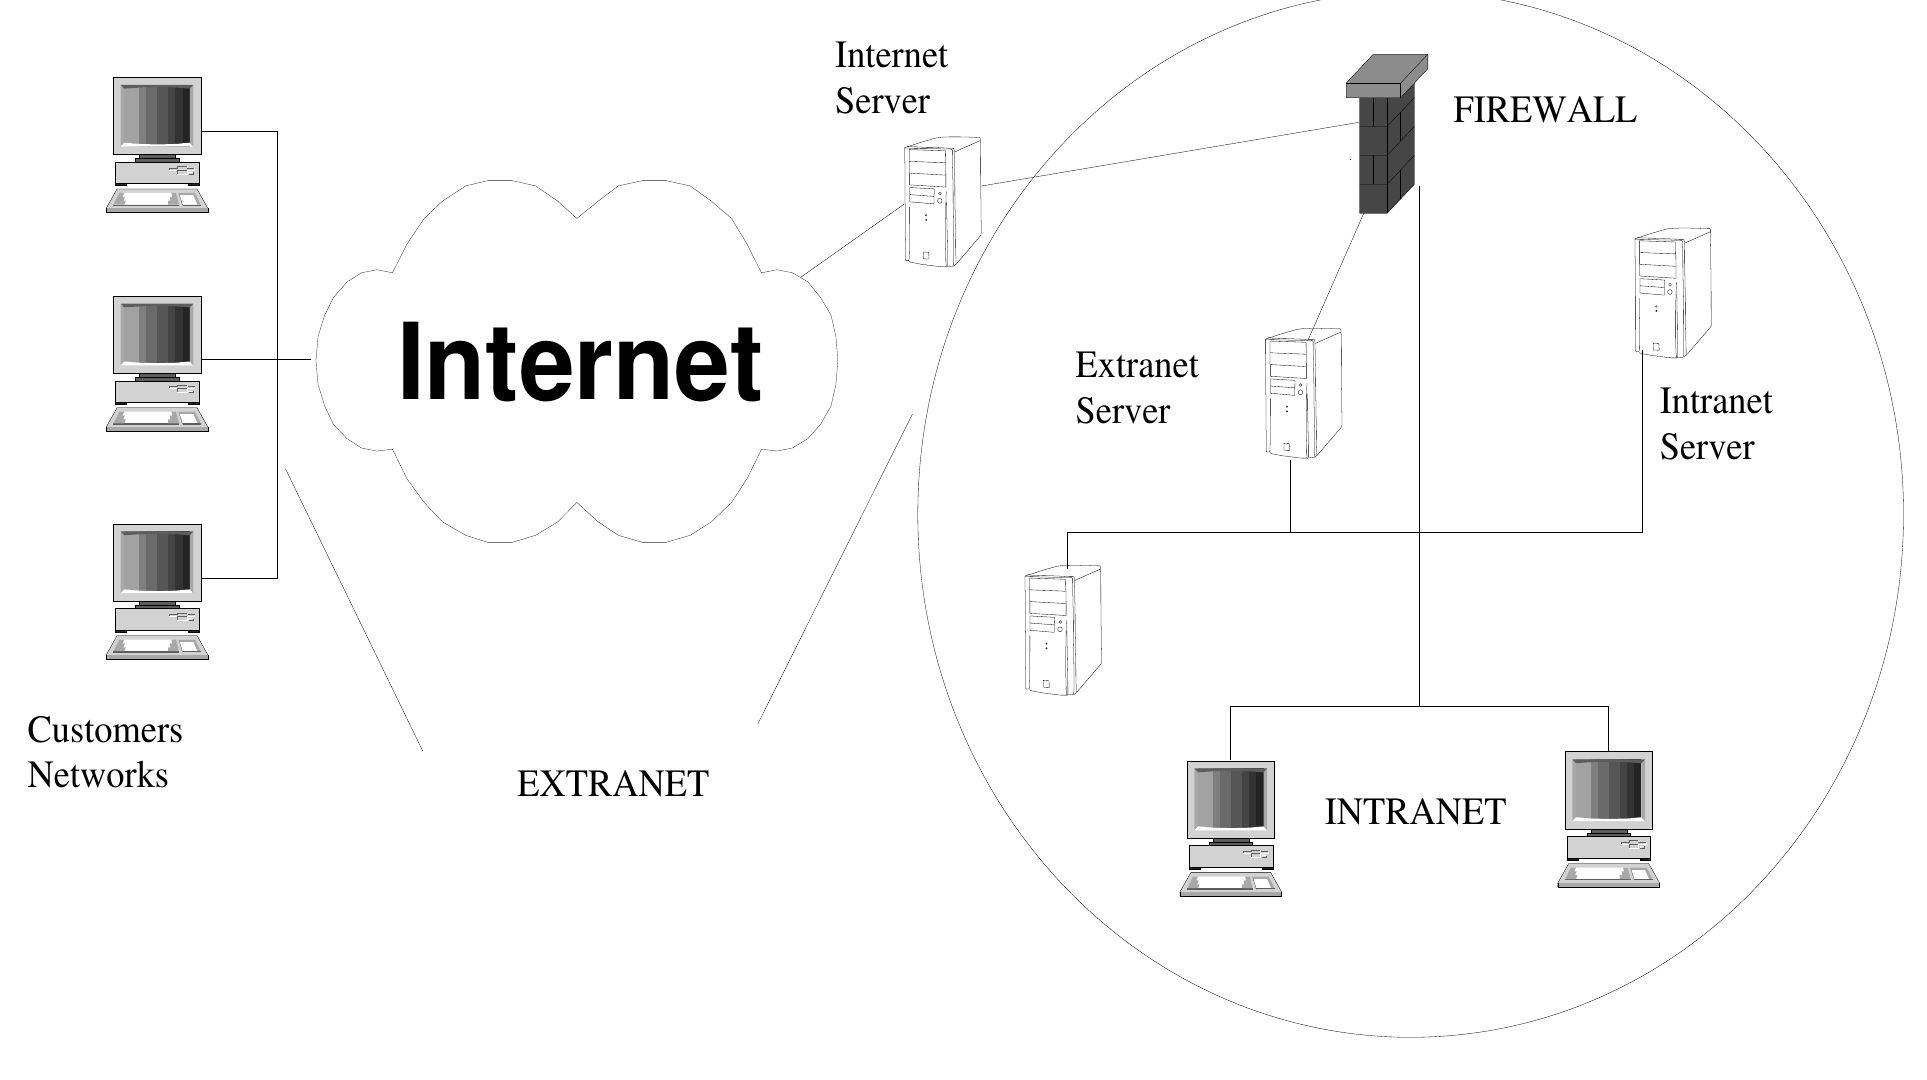
\includegraphics[width=\textwidth]{assets/images/fig11_1_extranet_cloud_topology.png}
  \caption{Những điểm tương đồng giữa một extranet an toàn và một Đám mây riêng}
  \label{fig:ch11_topology}
\end{figure}

Extranet là mạng máy tính được sử dụng bởi những người thuộc một mạng cụ thể với một định danh đăng nhập và mật khẩu. Chúng đôi khi được dùng bởi hai hay nhiều bộ phận để liên lạc với nhau hoặc bởi một số công ty để xử lý tài khoản cho những khách hàng cụ thể. Có ba yếu tố rủi ro đáng kể trong tình huống sử dụng này, được nêu ra như sau.

\textbf{Bảo đảm tính bí mật và tính toàn vẹn của dữ liệu đang truyền của tổ chức chúng ta đi tới và đi từ nhà cung cấp Đám mây công cộng:} Một số tài nguyên và dữ liệu trước đây bị giới hạn trong một mạng riêng nay lại bị phơi bày ra Internet, và ra một mạng công cộng chia sẻ thuộc về một nhà cung cấp Đám mây bên thứ ba. Mặc dù việc sử dụng HTTPS (thay vì HTTP) lẽ ra đã giảm thiểu được rủi ro về tính toàn vẹn, những người dùng không dùng HTTPS (mà dùng HTTP) đã phải đối mặt với rủi ro gia tăng rằng dữ liệu của họ có thể đã bị thay đổi trong quá trình truyền mà họ không hề hay biết.

\textbf{Bảo đảm kiểm soát truy cập phù hợp (xác thực, ủy quyền và kiểm toán) đối với bất kỳ tài nguyên nào mà chúng ta đang sử dụng tại nhà cung cấp Đám mây công cộng của bạn:} Bởi vì một tập con nào đó của các tài nguyên này (hoặc thậm chí có thể là toàn bộ chúng) nay đã bị phơi bày ra Internet, một tổ chức sử dụng Đám mây công cộng phải đối mặt với sự gia tăng đáng kể về rủi ro đối với dữ liệu của mình. Khả năng kiểm toán các hoạt động của mạng thuộc nhà cung cấp Đám mây của bạn (chưa nói đến việc tiến hành bất kỳ hoạt động giám sát thời gian thực nào, chẳng hạn như trên chính mạng của bạn), thậm chí là sau khi sự việc đã xảy ra, có lẽ là không tồn tại.

\textbf{Bảo đảm tính sẵn sàng của các tài nguyên hướng Internet trong một Đám mây công cộng đang được tổ chức chúng ta sử dụng, hoặc đã được các nhà cung cấp Đám mây công cộng gán cho tổ chức chúng ta:} Sự phụ thuộc vào bảo mật mạng đã tăng lên bởi vì một lượng dữ liệu gia tăng hoặc một số lượng nhân sự tổ chức gia tăng nay phụ thuộc vào các thiết bị được lưu trữ bên ngoài để bảo đảm tính sẵn sàng của các tài nguyên do Đám mây cung cấp.

Do đó, ba yếu tố rủi ro được liệt kê trong phần trên phải ở mức chấp nhận được đối với một tổ chức. Việc cấu hình sai (misconfiguration) vẫn có thể ảnh hưởng đến tính sẵn sàng của các tài nguyên dựa trên Đám mây của bạn.

Theo một nghiên cứu được trình bày trước Nhóm các nhà vận hành mạng Bắc Mỹ (North American Network Operators Group, NANOG) vào tháng 2 năm 2006, hàng trăm cấu hình sai như vậy xảy ra mỗi tháng. Ví dụ có lẽ nổi tiếng nhất về một sai lầm cấu hình như vậy đã xảy ra vào tháng 2 năm 2008 khi Pakistan Telecom mắc lỗi bằng cách công bố một tuyến giả (dummy route) cho YouTube tới đối tác viễn thông của chính mình là PCCW, có trụ sở tại Hồng Kông. Ý định là để chặn YouTube trong phạm vi Pakistan vì một số video bị cho là báng bổ được lưu trữ trên trang này. Kết quả là YouTube đã không thể truy cập được trên toàn cầu trong hai giờ.

\subsection{Bảo mật hạ tầng theo lược đồ vùng tin cậy (TZ)}

Tính dễ tổn thương của các Hệ thống điện toán đám mây (Cloud Computing Systems, CCS) trước các mối đe dọa dai dẳng nâng cao (advanced persistent threats, APT) là một mối quan ngại đáng kể đối với chính phủ và ngành công nghiệp. Nhân sự của Nhà cung cấp dịch vụ Đám mây (CSP) có quyền truy cập vật lý vào trung tâm dữ liệu của CSP có thể phá vỡ các biện pháp kiểm soát bảo mật bằng cách truy cập trực tiếp vào các máy vật lý. Tuy nhiên, số lượng lớn các máy làm phức tạp thêm nhiệm vụ này. Sự chính xác đòi hỏi kẻ tấn công trước tiên phải nhận diện được phần cứng đang lưu trữ dữ liệu mục tiêu. Kẻ nội gián của CSP không thể tiếp xúc vật lý với mọi máy trong trung tâm dữ liệu, nhưng anh ta có một vài phương pháp để định vị máy đang lưu trữ các máy ảo (VM) thuộc Vùng tin cậy (Trust Zones, TZ) của cơ quan.

TZ được định nghĩa là sự kết hợp giữa phân đoạn mạng (network segmentation) và các biện pháp kiểm soát quản lý danh tính và truy cập (identity and access management, IAM). Những thứ này định nghĩa các ranh giới vật lý, logic hoặc ảo xung quanh các tài nguyên mạng. Các TZ của Đám mây có thể được triển khai bằng các thiết bị vật lý, một cách ảo hóa bằng các ứng dụng tường lửa ảo và chuyển mạch ảo, hoặc bằng cả các thiết bị vật lý lẫn ảo. Bước đầu tiên là liệt kê tất cả các VM đang hoạt động của Cơ quan. Các máy chủ quản lý của CSP nắm giữ dữ liệu như vậy. Một quản trị viên hệ thống của CSP sẽ có quyền truy cập vào dữ liệu này.

Danh sách các VM của cơ quan có thể rất lớn. Kẻ tấn công phải thu hẹp danh sách lại để anh ta có thể tới thăm từng máy. Thông tin có thể giúp thu hẹp danh sách là dữ liệu cấu hình. Điều này bao gồm nhóm bảo mật (security group) và các cấu hình khác do bên thuê (tenant) tạo ra vốn tiết lộ tô-pô các tài nguyên của bên thuê trong Đám mây, các dịch vụ cụ thể có thể được suy đoán dựa trên những cổng cụ thể đang mở, dữ liệu quản lý danh tính và truy cập cho thấy những người dùng nào của bên thuê có tài khoản CSP và họ được phép làm gì với các tài nguyên cụ thể, các quy ước đặt tên của bên thuê cho các ảnh máy (machine image) hoặc thực thể (instance) của họ, và kích cỡ tương đối về bộ nhớ, đĩa, CPU và I/O của các thực thể khác nhau. Các bước này có khả năng nhận diện được, chẳng hạn, các máy lớn, vốn lưu trữ các tiến trình máy chủ web, chia sẻ tệp, hoặc cơ sở dữ liệu, và những máy có quyền truy cập bị hạn chế.

Một khi kẻ nội gián của CSP đã biết cần tới thăm những máy nào, anh ta phải ánh xạ những máy này vào sơ đồ bố trí của trung tâm dữ liệu. Những trung tâm dữ liệu được phân đoạn hoặc được ngăn thành các khoang, hoặc giữ riêng biệt quyền truy cập vào các bản đồ vật lý và logic, sẽ làm phức tạp thêm nhiệm vụ này. Ngược lại, những trung tâm dữ liệu có một điểm vào duy nhất sẽ khiến cuộc tấn công này dễ dàng hơn.

Mã độc được tiêm vào thông qua truy cập vật lý cung cấp một điểm đột phá cho kẻ tấn công. Bản thân sự đột phá này có thể cung cấp quyền truy cập mạng và các đặc quyền nâng cao trên bộ giám sát máy ảo (HV) đang lưu trữ VM mục tiêu. Bằng cách phát tín hiệu (beaconing) tới các nút điều khiển đã biết của kẻ tấn công, kẻ tấn công có thể thiết lập một liên kết để điều khiển việc thực thi phần còn lại của cuộc tấn công.

\section{Bảo mật ứng dụng PaaS}

Các nhà cung cấp PaaS nhìn chung rơi vào hai loại chính sau đây, tức là các nhà cung cấp phần mềm (ví dụ, Bungee, Etelos, GigaSpaces, Eucalyptus) và các CSP (ví dụ, Google App Engine, Force.com của Salesforce.com, Microsoft Azure, Intuit QuickBase).

Các tổ chức đang đánh giá một Đám mây riêng có thể sử dụng phần mềm PaaS để xây dựng một giải pháp cho việc tiêu dùng nội bộ. Hiện tại, không có Đám mây công cộng lớn nào được biết là đang sử dụng phần mềm PaaS thương mại có sẵn (commercial off-the-shelf) hoặc mã nguồn mở như Eucalyptus (Eucalyptus có cung cấp một Đám mây thử nghiệm thí điểm giới hạn dành cho các nhà phát triển tại Eucalyptus.com). Do đó, xét đến giai đoạn còn non trẻ của việc triển khai PaaS, khuyến nghị rằng các tổ chức đang đánh giá phần mềm PaaS nên thực hiện một đánh giá rủi ro và áp dụng tiêu chuẩn bảo mật phần mềm tương tự như khi mua sắm bất kỳ phần mềm doanh nghiệp nào.

Nói một cách tổng quát, các CSP của PaaS (ví dụ, Google, Microsoft và Force.com) chịu trách nhiệm bảo mật ngăn xếp phần mềm nền tảng, bao gồm cả bộ máy thực thi (runtime engine) chạy các ứng dụng của khách hàng. Bởi vì các ứng dụng PaaS có thể sử dụng các ứng dụng, thành phần hoặc dịch vụ web của bên thứ ba, nhà cung cấp ứng dụng bên thứ ba có thể phải chịu trách nhiệm bảo mật các dịch vụ của họ. Do đó, khách hàng nên hiểu rõ sự phụ thuộc của ứng dụng của mình vào tất cả các dịch vụ và đánh giá các rủi ro liên quan đến các nhà cung cấp dịch vụ bên thứ ba.

Cho đến nay, các CSP vẫn miễn cưỡng trong việc chia sẻ thông tin liên quan đến bảo mật nền tảng với lập luận rằng thông tin bảo mật như vậy có thể mang lại lợi thế cho tin tặc. Tuy nhiên, khách hàng doanh nghiệp nên đòi hỏi sự minh bạch từ các CSP và tìm kiếm thông tin cần thiết để thực hiện đánh giá rủi ro và quản lý bảo mật liên tục.

\subsection*{Kiểm soát truy cập PaaS}

Nói một cách tổng quát, quản lý kiểm soát truy cập trong PaaS là một chức năng rộng bao trùm các yêu cầu truy cập dành cho người dùng của bạn và các quản trị viên hệ thống (người dùng đặc quyền) vốn truy cập vào các tài nguyên mạng, hệ thống và ứng dụng. Các chức năng quản lý kiểm soát truy cập nên giải quyết những câu hỏi như: việc gán các quyền hạn (entitlement) cho người dùng, việc gán quyền hạn dựa trên chức năng công việc và trách nhiệm của người dùng, phương thức xác thực và mức độ mạnh yêu cầu trước khi cấp quyền truy cập vào tài nguyên, việc kiểm toán và báo cáo để xác minh các phân công quyền hạn. Những khía cạnh nêu trên của lĩnh vực kiểm soát truy cập nên được giải quyết bởi các chính sách và tiêu chuẩn truy cập của tổ chức và được điều chỉnh phù hợp với vai trò và trách nhiệm của người dùng, bao gồm cả người dùng cuối lẫn các quản trị viên hệ thống có đặc quyền.

\subsection*{Gia cố hệ điều hành máy chủ cho bảo mật PaaS}

Các lỗ hổng vốn có trong hệ điều hành của máy tính chủ (host) có thể lan ngược lên trên vào hệ điều hành của máy ảo. Trong khi một sự xâm phạm trên hệ điều hành của VM hy vọng chỉ làm tổn hại đến miền khách (guest domain), thì một sự xâm phạm của hệ điều hành chủ nền tảng sẽ cho kẻ xâm nhập quyền truy cập vào tất cả các dịch vụ trên tất cả các máy ảo được lưu trữ bởi máy đó. Do đó, các kỹ thuật gia cố theo thực hành tốt nhất phải được triển khai để duy trì trạng thái bảo mật của công nghệ nền tảng. Một số kỹ thuật này bao gồm những nội dung sau:

\begin{itemize}
  \item Sử dụng mật khẩu mạnh, chẳng hạn như mật khẩu dài, khó đoán với sự kết hợp của chữ cái, chữ số và ký hiệu, và thay đổi chúng thường xuyên.
  \item Vô hiệu hóa các dịch vụ hoặc chương trình không cần thiết, đặc biệt là các dịch vụ mạng.
  \item Yêu cầu xác thực đầy đủ cho việc kiểm soát truy cập.
  \item Máy chủ nên được đặt tường lửa riêng lẻ.
  \item Vá lỗi và cập nhật máy chủ thường xuyên, sau khi đã kiểm thử trên một đơn vị không thuộc môi trường sản xuất.
\end{itemize}

\subsection*{Lược đồ đăng nhập một lần (SSO) cho bảo mật PaaS}

Đăng nhập một lần (Single sign-on, SSO) giải quyết tình huống phiền toái của việc phải đăng nhập nhiều lần để truy cập các tài nguyên khác nhau. Khi người dùng phải ghi nhớ vô số mật khẩu và ID, họ có thể đi đường tắt trong việc tạo ra chúng, điều này có thể khiến họ dễ bị khai thác. Trong SSO, một người dùng cung cấp một ID và mật khẩu cho mỗi phiên làm việc và được tự động đăng nhập vào tất cả các ứng dụng cần thiết. Để bảo mật SSO, mật khẩu không nên được lưu trữ hoặc truyền đi ở dạng rõ.

Các ứng dụng SSO có thể chạy hoặc trên máy trạm của người dùng hoặc trên các máy chủ xác thực. Các ưu điểm của SSO bao gồm khả năng sử dụng mật khẩu mạnh hơn, việc quản trị thay đổi hoặc xóa mật khẩu dễ dàng hơn, và ít thời gian hơn để truy cập tài nguyên. Nhược điểm lớn của nhiều triển khai SSO là một khi người dùng đã có được quyền truy cập vào hệ thống thông qua lần đăng nhập ban đầu, họ có thể tự do đi lại trong các tài nguyên mạng mà không có bất kỳ hạn chế nào.

Một ví dụ rất phổ biến về đăng nhập SSO là triển khai của Google cho các sản phẩm phần mềm của họ. Một khi người dùng đã đăng nhập vào Gmail, người dùng tự động có được quyền truy cập vào YouTube, Google Drive, Google Photos và các sản phẩm khác của Google.

\section{Bảo mật ứng dụng SaaS}

Mô hình SaaS quy định rằng nhà cung cấp quản lý toàn bộ bộ ứng dụng được chuyển giao tới người dùng. Do đó, các nhà cung cấp SaaS phần lớn chịu trách nhiệm bảo mật các ứng dụng và thành phần mà họ cung cấp cho khách hàng. Khách hàng thường chịu trách nhiệm về các chức năng bảo mật vận hành, bao gồm quản lý người dùng và quản lý truy cập theo mức độ được nhà cung cấp hỗ trợ. Đó là một thông lệ phổ biến khi các khách hàng tiềm năng yêu cầu thông tin liên quan đến các thực hành bảo mật của nhà cung cấp. Thông tin này nên bao trùm thiết kế, kiến trúc, phát triển, kiểm thử bảo mật ứng dụng hộp đen và hộp trắng, và quản lý phát hành.

Một số ứng dụng SaaS, chẳng hạn như Google Apps, có các tính năng tích hợp sẵn mà người dùng cuối có thể gọi ra để gán quyền đọc và ghi cho những người dùng khác. Tuy nhiên, các tính năng quản lý đặc quyền có thể không phải là quyền truy cập nâng cao, chi tiết ở mức mịn (fine-grained) và có thể có những điểm yếu mà có thể không phù hợp với tiêu chuẩn kiểm soát truy cập của tổ chức bạn. Một ví dụ nắm bắt được vấn đề này là cơ chế mà Google Docs sử dụng trong việc xử lý các hình ảnh được nhúng trong tài liệu, cũng như các đặc quyền truy cập đối với các phiên bản cũ hơn của một tài liệu.

Rõ ràng là các hình ảnh được nhúng và lưu trữ trong Google Docs không được bảo vệ theo cùng cách mà một tài liệu được bảo vệ bằng các biện pháp kiểm soát chia sẻ. Điều đó có nghĩa là, nếu ai đó đã chia sẻ một tài liệu chứa các hình ảnh nhúng, thì người kia sẽ luôn có thể xem được những hình ảnh đó ngay cả sau khi bạn đã ngừng chia sẻ tài liệu.

\subsection{Lược đồ FHE cho bảo mật SaaS}

Không giống như mã hóa đồng cấu bộ phận (partially homomorphic encryption) vốn chỉ cho phép tính toán đồng cấu một số phép toán trên bản mã (ví dụ, phép cộng, phép nhân, các hàm bậc hai, v.v.), mã hóa đồng cấu toàn phần hỗ trợ việc tính toán tùy ý trên bản mã. Một lược đồ như vậy cho phép xây dựng các chương trình cho bất kỳ chức năng mong muốn nào, mà có thể được chạy trên các đầu vào đã mã hóa để tạo ra một bản mã của kết quả. Bởi vì một chương trình như vậy không bao giờ cần giải mã các đầu vào của nó, nó có thể được chạy bởi một bên không đáng tin cậy mà không tiết lộ các đầu vào và trạng thái nội bộ của nó.

Sau đây là một ví dụ rất đơn giản về cách một lược đồ mã hóa đồng cấu có thể hoạt động trong điện toán đám mây:

\begin{itemize}
  \item Doanh nghiệp B có một tập dữ liệu rất quan trọng (very important data set, VIDS) bao gồm các số 5 và 10. Để mã hóa tập dữ liệu, Doanh nghiệp B nhân mỗi phần tử trong tập với 2, tạo ra một tập mới mà các phần tử của nó là 10 và 20.
  \item Doanh nghiệp B gửi tập VIDS đã mã hóa lên Đám mây để lưu trữ an toàn. Vài tháng sau, chính phủ liên hệ với Doanh nghiệp X và yêu cầu tổng của các phần tử VIDS.
  \item Doanh nghiệp B rất bận, nên nó yêu cầu nhà cung cấp Đám mây thực hiện phép toán. Nhà cung cấp Đám mây, vốn chỉ có quyền truy cập vào tập dữ liệu đã mã hóa, tìm ra tổng của $10 + 20$ và trả về câu trả lời 30.
  \item Doanh nghiệp B giải mã câu trả lời của nhà cung cấp Đám mây và cung cấp cho chính phủ câu trả lời đã giải mã, 15.
\end{itemize}

\subsection*{Kiểm soát truy cập trong SaaS}

Trong một mô hình tiêu dùng điện toán đám mây, nơi người dùng đang truy cập các dịch vụ Đám mây từ bất kỳ máy chủ nào có kết nối Internet, kiểm soát truy cập mạng sẽ đóng một vai trò ngày càng suy giảm. Lý do là các biện pháp kiểm soát truy cập dựa trên mạng truyền thống tập trung vào việc bảo vệ tài nguyên khỏi sự truy cập trái phép dựa trên các thuộc tính của máy chủ, điều mà trong hầu hết các trường hợp là không thỏa đáng, không phải là duy nhất giữa các người dùng, và có thể gây ra việc hạch toán không chính xác. Trong Đám mây, kiểm soát truy cập mạng được thể hiện dưới dạng các chính sách tường lửa Đám mây thực thi kiểm soát truy cập dựa trên máy chủ tại các điểm vào và ra của Đám mây và việc nhóm các thực thể một cách logic bên trong Đám mây. Điều này thường đạt được bằng cách sử dụng các chính sách (quy tắc) sử dụng các tham số Giao thức điều khiển truyền vận/Giao thức Internet (Transmission Control Protocol/Internet Protocol, TCP/IP) tiêu chuẩn, bao gồm IP nguồn, cổng nguồn, IP đích và cổng đích.

Ngược lại với kiểm soát truy cập dựa trên mạng, kiểm soát truy cập người dùng nên được nhấn mạnh mạnh mẽ trong Đám mây, bởi vì nó có thể ràng buộc chặt chẽ danh tính của một người dùng với các tài nguyên trong Đám mây và sẽ hỗ trợ cho việc kiểm soát truy cập ở mức chi tiết mịn, hạch toán người dùng, hỗ trợ tuân thủ và bảo vệ dữ liệu. Các biện pháp kiểm soát quản lý truy cập người dùng, bao gồm xác thực mạnh, đăng nhập một lần (SSO), quản lý đặc quyền, cùng việc ghi nhật ký và giám sát các tài nguyên Đám mây, đóng một vai trò đáng kể trong việc bảo vệ tính bí mật và tính toàn vẹn của thông tin của bạn trong Đám mây. ISO/IEC 27002 đã định nghĩa sáu mục tiêu kiểm soát truy cập bao trùm kiểm soát truy cập của người dùng cuối, người dùng đặc quyền, mạng, ứng dụng và thông tin.

Tương tự như việc giám sát dịch vụ SaaS, các khách hàng đang lưu trữ ứng dụng trên một nền tảng IaaS nên thực hiện các bước bổ sung để giám sát tình trạng của ứng dụng được lưu trữ. Ví dụ, nếu chúng ta đang lưu trữ một ứng dụng thương mại điện tử trên một Đám mây ảo Amazon EC2, chúng ta nên giám sát tình trạng của cả ứng dụng thương mại điện tử lẫn các thực thể máy chủ ảo. Các chiến lược bảo mật máy chủ ảo được trình bày tiếp theo.

\section{Bảo mật máy chủ ảo}

Sự đơn giản của việc tự cấp phát (self-provisioning) các máy chủ ảo mới trên một nền tảng IaaS tạo ra một rủi ro rằng những máy chủ ảo không an toàn sẽ được tạo ra. Cấu hình an toàn theo mặc định (secure-by-default) cần phải được bảo đảm bằng cách tuân theo hoặc vượt qua các đường cơ sở (baseline) sẵn có của ngành. Việc bảo mật máy chủ ảo trong Đám mây đòi hỏi các thủ tục bảo mật vận hành mạnh mẽ kết hợp với việc tự động hóa các thủ tục. Sau đây là một số khuyến nghị từ các tổ chức CNTT.

\textbf{Sử dụng cấu hình an toàn theo mặc định:} Ảnh VM phải được gia cố và được sử dụng như một ảnh gia cố tiêu chuẩn để tạo thực thể các VM (hệ điều hành khách) trong một Đám mây công cộng. Một thực hành tốt nhất cho các ứng dụng dựa trên Đám mây là xây dựng các ảnh VM tùy chỉnh chỉ có những khả năng và dịch vụ cần thiết để hỗ trợ ngăn xếp ứng dụng. Việc giới hạn các khả năng của ngăn xếp ứng dụng nền tảng không chỉ giới hạn bề mặt tấn công tổng thể của máy chủ, mà còn giảm đáng kể số lượng bản vá cần thiết để giữ cho ngăn xếp ứng dụng đó được an toàn.

\textbf{Theo dõi kiểm kê các ảnh VM và các phiên bản hệ điều hành đã được chuẩn bị cho việc lưu trữ trên Đám mây:} Nhà cung cấp IaaS cung cấp một số trong các ảnh VM này. Khi một ảnh ảo từ nhà cung cấp IaaS được sử dụng, nó nên trải qua cùng mức độ xác minh bảo mật và gia cố như đối với các máy chủ bên trong doanh nghiệp. Phương án thay thế tốt nhất là cung cấp ảnh của chính bạn vốn tuân thủ cùng các tiêu chuẩn bảo mật như các máy chủ nội bộ đáng tin cậy. Hãy bảo vệ tính toàn vẹn của ảnh đã gia cố khỏi sự truy cập trái phép.

\textbf{Bảo vệ các khóa riêng cần thiết để truy cập các máy chủ trong Đám mây công cộng:} Nói chung, việc cô lập các khóa giải mã khỏi Đám mây nơi dữ liệu được lưu trữ là điều bắt buộc, trừ khi chúng là cần thiết cho việc giải mã. Nếu một ứng dụng đòi hỏi một khóa để mã hóa và giải mã cho việc xử lý dữ liệu liên tục, thì có thể sẽ không thể bảo vệ được khóa đó bởi vì nó sẽ nằm cùng chỗ với ứng dụng.

\textbf{Không bao gồm chứng thư xác thực nào trong các ảnh ảo hóa ngoại trừ một khóa để giải mã khóa hệ thống tệp:} Chúng ta không nên cho phép xác thực dựa trên mật khẩu đối với truy cập shell. Đối với các đặc quyền quản trị (\texttt{sudo *}) hoặc truy cập dựa trên vai trò (ví dụ, Solaris, SELinux), mật khẩu là bắt buộc.

\textbf{Chạy một tường lửa máy chủ và chỉ mở tối thiểu các cổng cần thiết để hỗ trợ các dịch vụ trên một thực thể:} Người dùng chỉ nên chạy các dịch vụ cần thiết và tắt các dịch vụ không sử dụng (ví dụ, tắt FTP, dịch vụ in, dịch vụ tệp mạng và dịch vụ cơ sở dữ liệu nếu chúng không được yêu cầu).

\textbf{Bật kiểm toán hệ thống và ghi nhật ký sự kiện, và ghi các sự kiện bảo mật vào một máy chủ nhật ký chuyên dụng:} Máy chủ nhật ký với mức bảo vệ bảo mật cao hơn, bao gồm cả kiểm soát truy cập, cần phải được cô lập.

\section{Các biện pháp kiểm soát bảo mật đám mây}

Kiến trúc bảo mật Đám mây chỉ hiệu quả nếu các triển khai phòng thủ đúng đắn được đặt đúng chỗ. Một kiến trúc bảo mật Đám mây hiệu quả nên nhận diện được các vấn đề sẽ nảy sinh cùng với việc quản lý bảo mật. Việc quản lý bảo mật giải quyết những vấn đề này bằng các biện pháp kiểm soát bảo mật (security control). Các biện pháp kiểm soát này được đặt ra để bảo vệ bất kỳ điểm yếu nào trong hệ thống và giảm bớt tác động của một cuộc tấn công. Mặc dù có nhiều loại biện pháp kiểm soát đằng sau một kiến trúc bảo mật Đám mây, chúng thường có thể được tìm thấy trong một trong các loại sau đây.

\textbf{Biện pháp kiểm soát răn đe (Deterrent controls):} Những biện pháp kiểm soát này nhằm mục đích làm giảm các cuộc tấn công vào một hệ thống Đám mây. Giống như một biển cảnh báo trên hàng rào hay trên một tài sản, các biện pháp kiểm soát răn đe thường làm giảm mức độ đe dọa bằng cách thông báo cho những kẻ tấn công tiềm năng rằng sẽ có những hậu quả bất lợi dành cho chúng nếu chúng tiếp tục.

\textbf{Biện pháp kiểm soát phòng ngừa (Preventive controls):} Nó tăng cường hệ thống chống lại các sự cố, nói chung bằng cách giảm thiểu nếu không muốn nói là loại bỏ hẳn các lỗ hổng. Chẳng hạn, việc xác thực mạnh đối với người dùng Đám mây khiến cho khả năng người dùng trái phép có thể truy cập các hệ thống Đám mây trở nên ít hơn, và khả năng người dùng Đám mây được nhận diện một cách chắc chắn trở nên cao hơn.

\textbf{Biện pháp kiểm soát phát hiện (Detective controls):} Các biện pháp kiểm soát phát hiện nhằm mục đích phát hiện và phản ứng một cách phù hợp với bất kỳ sự cố nào xảy ra. Trong trường hợp có một cuộc tấn công, một biện pháp kiểm soát phát hiện sẽ báo hiệu cho các biện pháp kiểm soát phòng ngừa hoặc khắc phục để giải quyết vấn đề. Việc giám sát bảo mật hệ thống và mạng, bao gồm các cơ chế phát hiện và ngăn chặn xâm nhập, thường được sử dụng để phát hiện các cuộc tấn công vào các hệ thống Đám mây và hạ tầng truyền thông hỗ trợ.

\textbf{Biện pháp kiểm soát khắc phục (Corrective controls):} Nó làm giảm hậu quả của một sự cố, thường bằng cách giới hạn thiệt hại. Chúng có hiệu lực trong hoặc sau một sự cố. Việc khôi phục các bản sao lưu hệ thống nhằm tái dựng lại một hệ thống đã bị xâm phạm là một ví dụ về biện pháp kiểm soát khắc phục.

\backsection{Tóm tắt}

Điện toán đám mây là một mô hình còn non trẻ và đang tiến hóa nhanh chóng, với các khía cạnh và khả năng mới được công bố thường xuyên. Trong chương này, chúng tôi cung cấp một cái nhìn toàn diện và kịp thời về các vấn đề bảo mật liên quan đến các dịch vụ IaaS, PaaS và SaaS. Các tổ chức chỉ dựa hoàn toàn vào bảo mật tích hợp sẵn của một nhà cung cấp Đám mây có khả năng phơi bày tổ chức của mình trước những rủi ro không cần thiết. Điều này đặc biệt đúng đối với các chứng thư (credential) và các bí mật (secret) vốn sinh sôi nảy nở trong các môi trường Đám mây và các quy trình tự động hóa. Những bí mật này được tạo ra một cách động và được gán để cấp phát, cấu hình và quản lý hàng trăm nghìn máy và vi dịch vụ (microservice), nhưng nhiều trong số chúng không bao giờ được bảo mật. Nếu chúng bị xâm phạm, những bí mật và chứng thư này có thể trao cho kẻ tấn công một điểm xuất phát then chốt để đạt được quyền truy cập theo chiều ngang (lateral access) xuyên qua các mạng, dữ liệu và ứng dụng, và cuối cùng, cung cấp quyền truy cập vào những tài sản quan trọng nhất của một tổ chức.

\backsection{Từ khóa}

\noindent
\begin{tabular}{@{}p{0.46\linewidth}@{\hspace{2em}}p{0.46\linewidth}@{}}
Quản lý bảo mật (Security management) & Bảo mật dữ liệu (Data security) \\[4pt]
Bảo mật IaaS (IaaS security)          & Bảo mật PaaS (PaaS security)   \\[4pt]
Bảo mật SaaS (SaaS security)          &                                 \\
\end{tabular}

\backsection{Câu hỏi trắc nghiệm}

\mcq{1. Nhà cung cấp dịch vụ nào sau đây cung cấp mức bảo mật tích hợp sẵn ít nhất?}
{(a) SaaS}
{(b) PaaS}
{(c) IaaS}
{(d) Tất cả các đáp án trên}

\mcq{2. Hãy chỉ ra phát biểu đúng:}
{(a) Các loại mô hình dịch vụ điện toán đám mây khác nhau cung cấp các mức dịch vụ bảo mật khác nhau}
{(b) Việc điều chỉnh các hệ thống tại chỗ (on-premises) của bạn sang một mô hình Đám mây đòi hỏi bạn phải xác định những cơ chế bảo mật nào là cần thiết và ánh xạ chúng vào các biện pháp kiểm soát đang tồn tại ở nhà cung cấp dịch vụ Đám mây mà bạn đã chọn}
{(c) Dữ liệu nên được truyền và lưu trữ ở định dạng đã mã hóa nhằm mục đích bảo mật}
{(d) Tất cả các đáp án trên}

\mcq{3. Dịch vụ nào sau đây cần được thương lượng trong các Thỏa thuận mức dịch vụ (\textenglish{Service Level Agreement})?}
{(a) Ghi nhật ký (Logging)}
{(b) Kiểm toán (Auditing)}
{(c) Tuân thủ quy định (Regulatory compliance)}
{(d) Tất cả các đáp án trên}

\mcq{4. Hãy chỉ ra phát biểu sai:}
{(a) Bạn có thể sử dụng các dịch vụ proxy và môi giới (brokerage) để tách các máy khách khỏi việc truy cập trực tiếp vào bộ nhớ Đám mây được chia sẻ}
{(b) Bất kỳ ứng dụng phân tán nào cũng có bề mặt tấn công lớn hơn nhiều so với một ứng dụng được giữ chặt trong một mạng LAN}
{(c) Điện toán đám mây không có các lỗ hổng liên quan đến các ứng dụng Internet}
{(d) Tất cả các đáp án trên}

\mcq{5. Lĩnh vực nào sau đây của điện toán đám mây là đặc biệt rắc rối?}
{(a) Kiểm toán (Auditing)}
{(b) Toàn vẹn dữ liệu (Data integrity)}
{(c) e-Discovery cho tuân thủ pháp lý}
{(d) Tất cả các đáp án trên}

\mcq{6. Điều nào sau đây là lĩnh vực vận hành (operational domain) của CSA?}
{(a) Khả năng mở rộng (Scalability)}
{(b) Tính khả chuyển và khả năng tương tác (Portability and interoperability)}
{(c) Tính linh hoạt (Flexibility)}
{(d) Không đáp án nào ở trên}

\mcq{7. Điều nào sau đây được CSA coi là một yếu tố thiết yếu trong điện toán đám mây?}
{(a) Đa thuê bao (Multi-tenancy)}
{(b) Quản lý danh tính và truy cập (Identity and access management)}
{(c) Ảo hóa (Virtualization)}
{(d) Tất cả các đáp án trên}

\mcq{8. Điều nào sau đây được dùng cho quản lý hiệu năng Web và kiểm thử tải?}
{(a) VMware Hyperic}
{(b) Webmetrics}
{(c) Univa UD}
{(d) Tapinsystems}

\mcq{9. Điều nào sau đây là phần mềm quản lý ứng dụng và hạ tầng cho các Đám mây lai đa Đám mây (hybrid multi-Clouds)?}
{(a) VMware Hyperic}
{(b) Webmetrics}
{(c) Univa UD}
{(d) Tapinsystems}

\mcq{10. Điều nào sau đây là dịch vụ bảo mật XML dựa trên chính sách của Cisco?}
{(a) Application Oriented Manager}
{(b) Application Oriented Networking}
{(c) Application Process Networking}
{(d) Tất cả các đáp án trên}

\mcq{11. Hãy chỉ ra phát biểu sai:}
{(a) SOA loại bỏ việc sử dụng các ranh giới ứng dụng, các phương pháp truyền thống trong đó bảo mật ở mức ứng dụng có khả năng không còn hiệu quả}
{(b) Một dịch vụ nguyên tử (atomic service) không thể được phân rã thành các dịch vụ nhỏ hơn mà vẫn cung cấp một chức năng hữu ích}
{(c) Dịch vụ bảo mật XML có thể được tìm thấy trong NetScaler 9.0 của Citrix}
{(d) Không đáp án nào ở trên}

\mcq{12. Điều nào sau đây không phải là một chuẩn OASIS cho bảo mật SOA?}
{(a) Security Assertion Markup Language}
{(b) \textenglish{Synchronized Multimedia Integration Language}}
{(c) WS-SecureConversion}
{(d) Tất cả các đáp án trên}

\mcq{13. Điều nào sau đây cung cấp xác thực và ủy quyền dữ liệu giữa máy khách và dịch vụ?}
{(a) SAML}
{(b) WS-SecureConversion}
{(c) WS-Security}
{(d) Tất cả các đáp án trên}

\mcq{14. Hãy chỉ ra phát biểu sai:}
{(a) Để giải quyết bảo mật SOA, một tập các chuẩn OASIS đã được tạo ra}
{(b) WS-SecureConversion gắn một mã thông báo ngữ cảnh bảo mật (security context token) vào các hoạt động truyền thông chẳng hạn như SOAP vốn được dùng để vận chuyển thông điệp trong một doanh nghiệp SOA}
{(c) WS-Trust là một phần mở rộng của SOA nhằm thực thi bảo mật bằng cách áp dụng các mã thông báo như Kerberos, SAML, hoặc X.509 vào các thông điệp}
{(d) Không đáp án nào ở trên}

\mcq{15. Điều nào sau đây là giao thức dịch vụ web để tạo và chia sẻ ngữ cảnh bảo mật?}
{(a) WS-Trust}
{(b) WS-Secure Conversion}
{(c) WS-Security Policy}
{(d) Tất cả các đáp án trên}

\backsection{Câu hỏi trắc nghiệm: đáp án}

\noindent 1:c \quad 2:d \quad 3:d \quad 4:c \quad 5:d \quad 6:b \quad 7:a \quad 8:b \quad 9:c \quad 10:b \quad 11:d \quad 12:b \quad 13:a \quad 14:c \quad 15:b

\backsection{Câu hỏi ôn tập}

\begin{enumerate}
  \item Một nhà cung cấp dịch vụ Đám mây bảo đảm tính toàn vẹn dữ liệu trong quá trình truyền tải (bên trong các Đám mây và trên đường đi từ/đến Đám mây) như thế nào?
  \item Dữ liệu và ứng dụng của một khách hàng được tách biệt khỏi dữ liệu và ứng dụng của các khách hàng khác như thế nào?
  \item Các nhà cung cấp áp dụng các luật lệ và quy định có thể áp dụng cho điện toán đám mây như thế nào?
  \item Hãy nêu các nền tảng được sử dụng cho điện toán đám mây quy mô lớn.
  \item Sự khác biệt giữa điện toán đám mây và điện toán cho thiết bị di động là gì?
  \item Người dùng có thể thu được lợi ích gì từ điện toán tiện ích (utility computing)?
  \item Các khía cạnh bảo mật được cung cấp cùng với Đám mây là gì?
  \item Hãy liệt kê các tầng khác nhau định nghĩa nên kiến trúc Đám mây.
  \item ``EUCALYPTUS'' là viết tắt của cái gì?
  \item Yêu cầu về nền tảng ảo hóa trong việc triển khai Đám mây là gì?
  \item Hãy nêu tên một số nhà cung cấp Đám mây và cơ sở dữ liệu lớn.
  \item Hãy giải thích sự khác biệt giữa Đám mây và các trung tâm dữ liệu truyền thống?
\end{enumerate}

\backsection{Câu hỏi tư duy phản biện}

\begin{enumerate}
  \item Hãy tìm kiếm trong tài liệu các bài báo đề xuất một kiến trúc phân tầng cho các Đám mây tính toán và phân tích một cách phản biện tính thực tiễn của mỗi cách tiếp cận này.
  \item Hãy thảo luận các phương tiện để đối phó với sự phức tạp của các hệ thống máy tính và truyền thông ngoài mô-đun hóa (modularity), phân tầng (layering) và phân cấp (hierarchy).
  \item Chúng ta biết rằng một VMBK (Virtual Machine-Based Rootkit, Rootkit dựa trên máy ảo) có thể gây ra những vấn đề bảo mật nghiêm trọng như thế nào. Hãy đưa ra các ví dụ khác trong đó sự trừu tượng hóa của một hệ thống vật lý có thể bị khai thác cho các hoạt động bất chính.
  \item Hãy đưa ra các ví dụ về hành vi không mong muốn của hệ thống tính toán và truyền thông mà có thể được đặc trưng hóa như các chuyển pha (phase transition). Bạn có thể hình dung ra một chuyển pha trong một Đám mây không?
\end{enumerate}

\begin{thebibliography}{99}

\bibitem{ch11-1} Chen H, Liu X, Xu H, Wang C, ``A Cloud service broker based on dynamic game theory for bilateral SLA negotiation in Cloud environment'', \textit{Int J Grid Distrib Comput}, Vol. 9, no. 9, 2018, pp. 251--268.

\bibitem{ch11-2} R. Gellman, ``Privacy in the Clouds: Risks to privacy and confidentiality from Cloud computing'', \textit{The World Privacy Forum}, 2009, Available at: \url{http://www.worldprivacyforum.org/}

\bibitem{ch11-3} Ohlman, B., Eriksson, A., Rembarz, R., ``What Networking of Information Can Do for Cloud Computing'', \textit{Proceedings of 18th IEEE International Workshops on Enabling Technologies: Infrastructures for Collaborative Enterprises}, Groningen, The Netherlands, June 29--July 1, 2009.

\bibitem{ch11-4} L. J. Zhang and Qun Zhou, ``CCOA: Cloud Computing Open Architecture'', \textit{IEEE International Conference on Web Services}, pp. 607--616, 2009.

\bibitem{ch11-5} Tim Mather, Subra Kumaraswamy, Shahed Latif, ``Cloud Security and Privacy: An Enterprise Perspective on Risks and Compliance'', Book published by O'Reilly Media, USA, 2009.

\bibitem{ch11-6} Ronald L. Krutz, Russell Dean Vines, ``Cloud Security: A Comprehensive Guide to Secure Cloud Computing'', Book published by Wiley Publishing Inc., 2010.

\bibitem{ch11-7} K. Vieira, A. Schulter, C. B. Westphall, and C. M. Westphall, ``Intrusion detection techniques for Grid and Cloud Computing Environment'', \textit{IT Professional Magazine}, IEEE Computer Society, Vol. 12, no. 4, pp. 38--43, 2010.

\bibitem{ch11-8} Marios D. Dikaiakos, Dimitrios Katsaros, Pankaj Mehra, George Pallis, Athena Vakali, ``Cloud Computing: Distributed Internet Computing for IT and Scientific Research'', \textit{IEEE Internet Computing Journal}, Vol. 13, no. 5, pp. 10--13, September 2009, DOI: 10.1109/MIC.2009.103.

\bibitem{ch11-9} A. Williamson, ``Comparing Cloud computing providers'', \textit{Cloud Comp. Journal}, Vol. 2, no. 3, pp. 3--5, 2009.

\end{thebibliography}
